\documentclass[11pt,letterpaper]{article}
\usepackage[top=3cm, bottom=2cm, left=2cm, right=2cm, columnsep=20pt]{geometry}
\usepackage{pdfpages}
\usepackage{graphicx}
\usepackage{etoolbox}
\apptocmd{\sloppy}{\hbadness 10000\relax}{}{}
% \usepackage[numbers]{natbib}
\usepackage[T1]{fontenc}
\usepackage{ragged2e}
\usepackage[french]{babel}
\usepackage{listings}
\usepackage{color}
\usepackage{soul}
\usepackage[utf8]{inputenc}
\usepackage[export]{adjustbox}
\usepackage{caption}
\usepackage{amsmath}
\usepackage{amssymb}
\usepackage{float}
\usepackage{csquotes}
\usepackage{fancyhdr}
\usepackage{wallpaper}
\usepackage{siunitx}
\usepackage[indent]{parskip}
\usepackage{textcomp}
\usepackage{gensymb}
\usepackage{multirow}
\usepackage[hidelinks]{hyperref}
\usepackage{abstract}
\renewcommand{\abstractnamefont}{\normalfont\bfseries}
\renewcommand{\abstracttextfont}{\normalfont\itshape}
\usepackage{titlesec}
\titleformat{\section}{\large\bfseries}{\thesection}{1em}{}
\titleformat{\subsection}{\normalsize\bfseries}{\thesubsection}{1em}{}
\titleformat{\subsubsection}{\normalsize\bfseries}{\thesubsubsection}{1em}{}

\usepackage{xcolor}
\definecolor{codegreen}{rgb}{0,0.6,0}
\definecolor{codegray}{rgb}{0.5,0.5,0.5}
\definecolor{codepurple}{rgb}{0.58,0,0.82}
\definecolor{backcolour}{rgb}{0.95,0.95,0.92}
\lstdefinestyle{mystyle}{
    backgroundcolor=\color{backcolour},   
    commentstyle=\color{codegreen},
    keywordstyle=\color{magenta},
    numberstyle=\tiny\color{codegray},
    stringstyle=\color{codepurple},
    basicstyle=\ttfamily\footnotesize,
    breakatwhitespace=false,         
    breaklines=true,                 
    captionpos=b,                    
    keepspaces=true,                 
    numbers=left,                    
    numbersep=5pt,                  
    showspaces=false,                
    showstringspaces=false,
    showtabs=false,                  
    tabsize=2
}
\lstset{style=mystyle}

\usepackage[most]{tcolorbox}
\newtcolorbox{note}[1][]{
  enhanced jigsaw,
  borderline west={2pt}{0pt}{black},
  sharp corners,
  boxrule=0pt, 
  fonttitle={\large\bfseries},
  coltitle={black},
  title={Note:\ },
  attach title to upper,
  #1
}

%----------------------------------------------------

\setlength{\parindent}{0pt}
\DeclareCaptionLabelFormat{mycaptionlabel}{#1 #2}
\captionsetup[figure]{labelsep=colon}
\captionsetup{labelformat=mycaptionlabel}
\captionsetup[figure]{name={Figure }}
\newcommand{\inlinecode}{\normalfont\texttt}
\usepackage{enumitem}
\setlist[itemize]{label=\textbullet}

\begin{document}
\begin{titlepage}
\center

\begin{figure}
    \ThisULCornerWallPaper{.4}{Polytechnique_signature-RGB-gauche_FR.png}
\end{figure}
\vspace*{2 cm}

\textsc{\Large \textbf{PHS2223 --} Introduction à l'optique moderne}\\[0.5cm]
\large{\textbf{Équipe : 04}}\\[1.5cm]

\rule{\linewidth}{0.5mm} \\[0.5cm]
\Large{\textbf{Expérience 4}} \\[0.2cm]
\text{Filtrage spatial}\\
\rule{\linewidth}{0.2mm} \\[2.3cm]

\large{\textbf{Présenté à}\\
  Guillaume Sheehy\\
  Esmat Zamani\\[2.5cm]
  \textbf{Par :}\\
  Émile \textbf{Guertin-Picard} (2208363)\\
  Laura-Li \textbf{Gilbert} (2204234)\\
  Tom \textbf{Dessauvages} (2133573)\\[3cm]}

\large{\today\\
Département de Génie Physique\\
Polytechnique Montréal\\}

\end{titlepage}

%----------------------------------------------------

\tableofcontents
\pagenumbering{roman}
\newpage

\pagestyle{fancy}
\setlength{\headheight}{14pt}
\renewcommand{\headrulewidth}{0pt}
\fancyfoot[R]{\thepage}

\pagestyle{fancy}
\fancyhf{}
\renewcommand{\headrulewidth}{1pt}
\fancyhead[L]{\textbf{PHS2223}}
\fancyhead[C]{Rapport final}
\fancyhead[R]{\today}
\fancyfoot[R]{\thepage}

\pagenumbering{arabic}
\setcounter{page}{1}

%----------------------------------------------------

\section{Résultats}

Cette section présente tous les résultats des manipulations, soit les images prises de l'acétate de Marvin
ainsi que de la cible de résolution.

\subsection{Cibles de résolution}

Pour les cibles de résolution des figures \ref{cible1.2} à \ref{cible25}, les fréquences de coupure ont été identifiées en déterminant la
valeur de fréquence spatiale la plus petite où les barres verticales étaient toujours distinguables.

\begin{figure}[H]
  \centering
  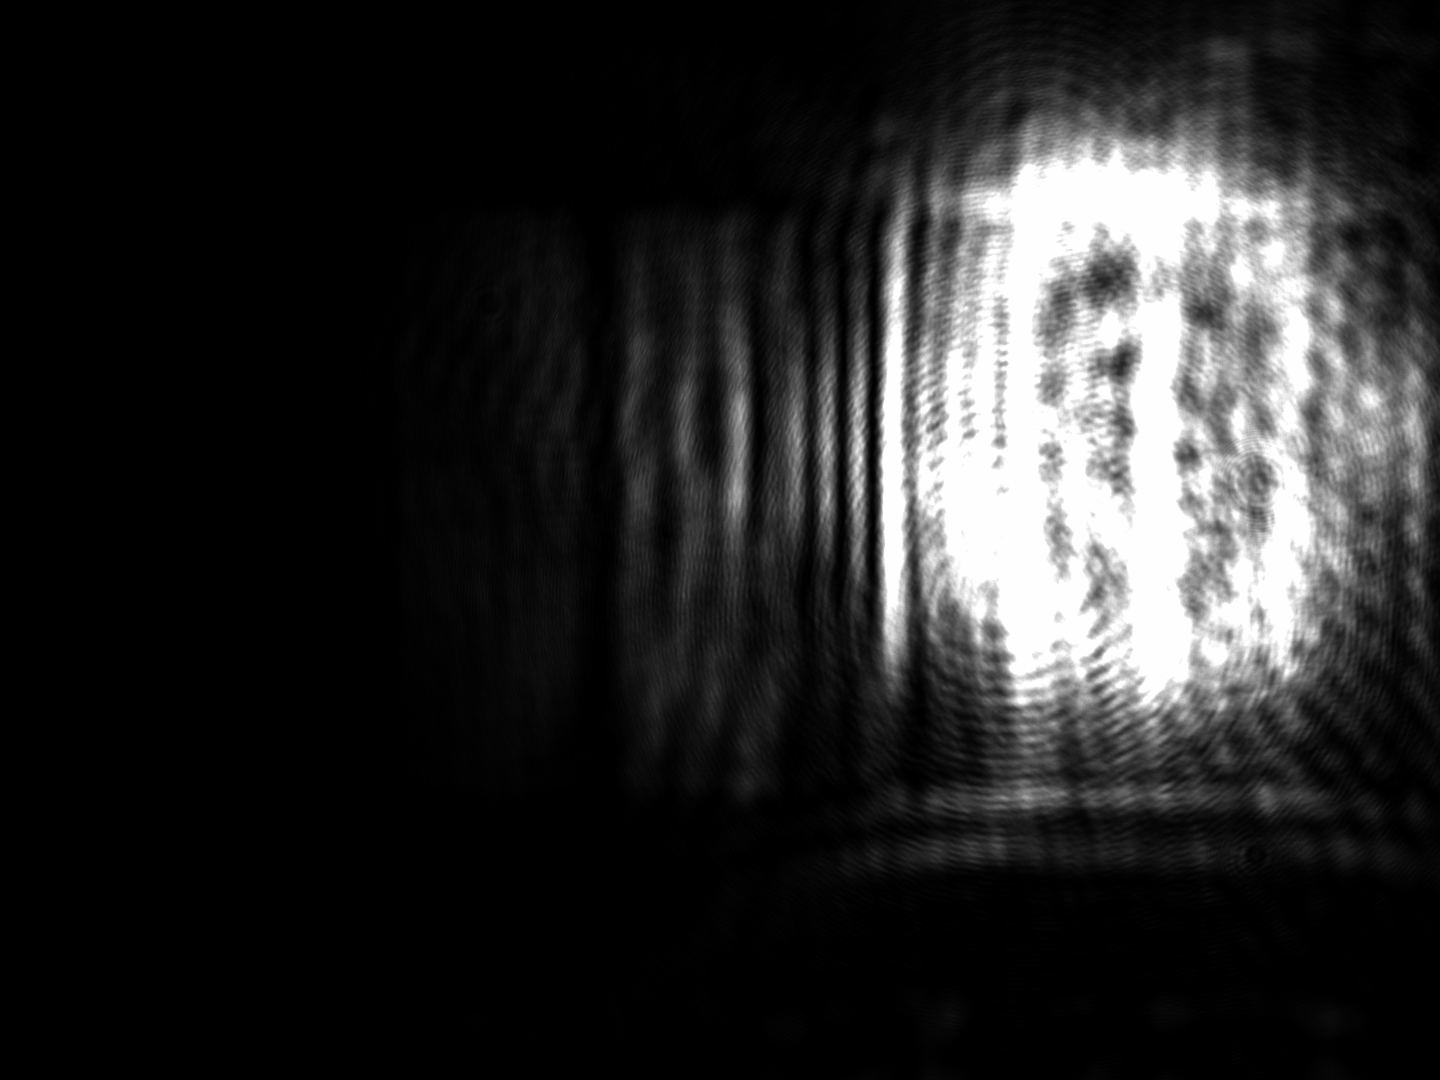
\includegraphics[scale=0.26]{cible_d1.2_1-7.png}
  \caption{Cible de résolution entre 1.25 et 3.85 mm$^{-1}$ pour un diamètre d'ouverture de l'iris de 1 mm. La fréquence de coupure est identifiée au minimum, soit 1.25 mm$^{-1}$.}
  \label{cible1.2}
\end{figure}

\begin{figure}[H]
  \centering
  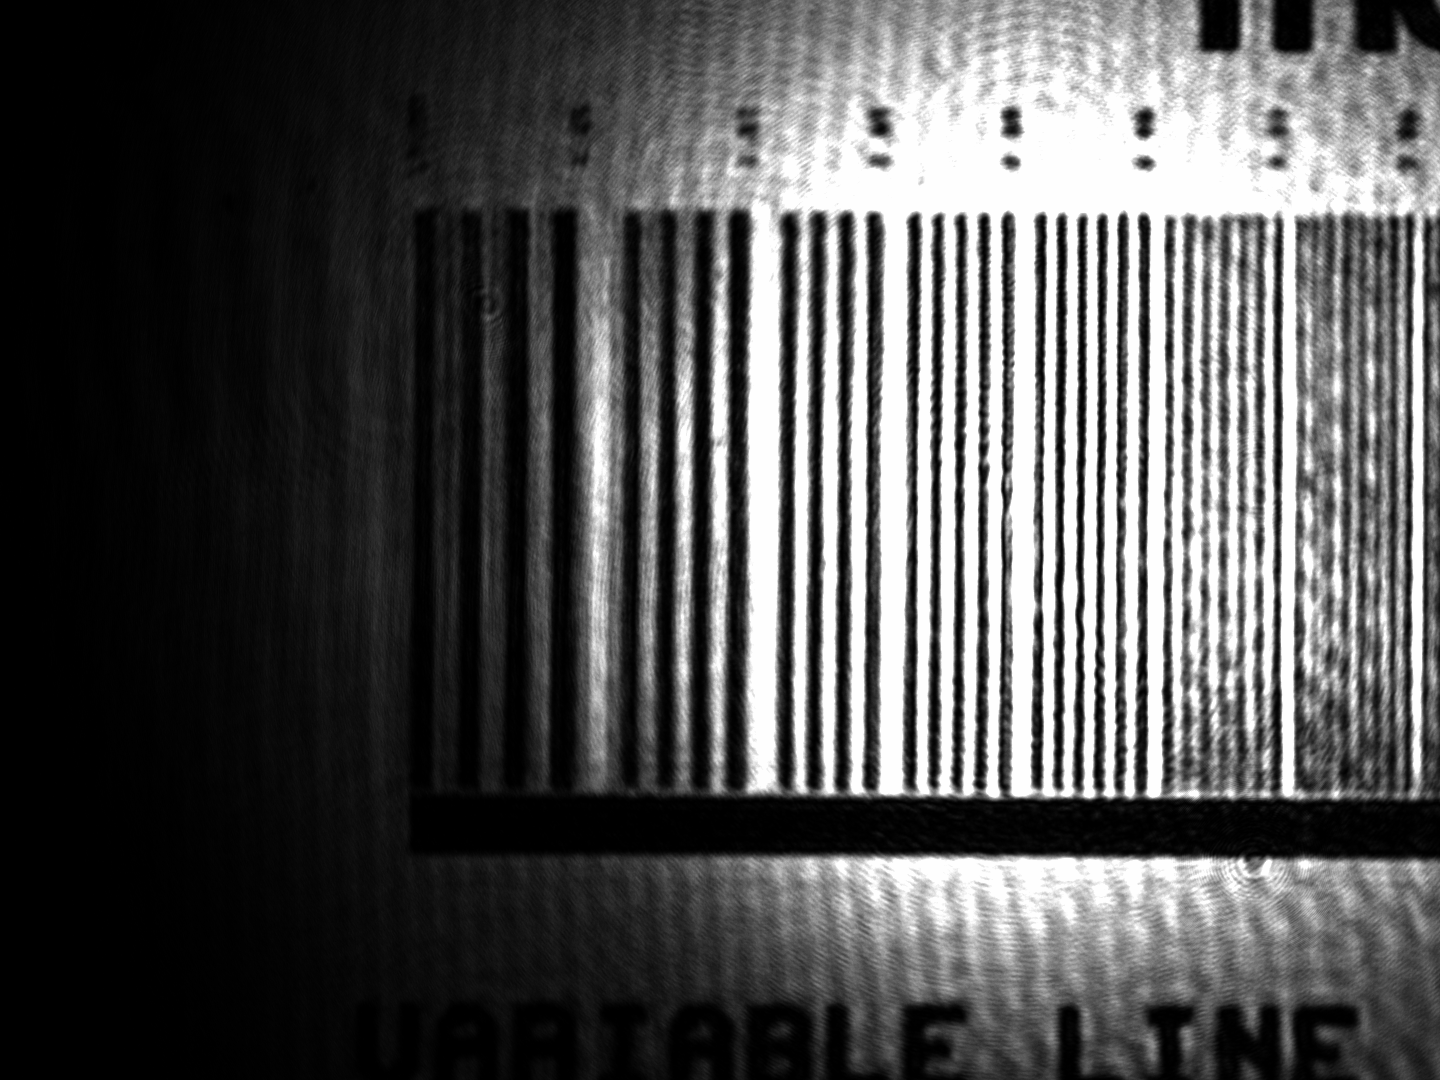
\includegraphics[scale=0.26]{cible_d2_1-7.png}
  \caption{Cible de résolution entre 1.25 et 3.85 mm$^{-1}$ pour un diamètre d'ouverture de l'iris de 2 mm. La fréquence de coupure est identifiée à 3.33 mm$^{-1}$.}
  \label{cible2}
\end{figure}

\begin{figure}[H]
  \centering
  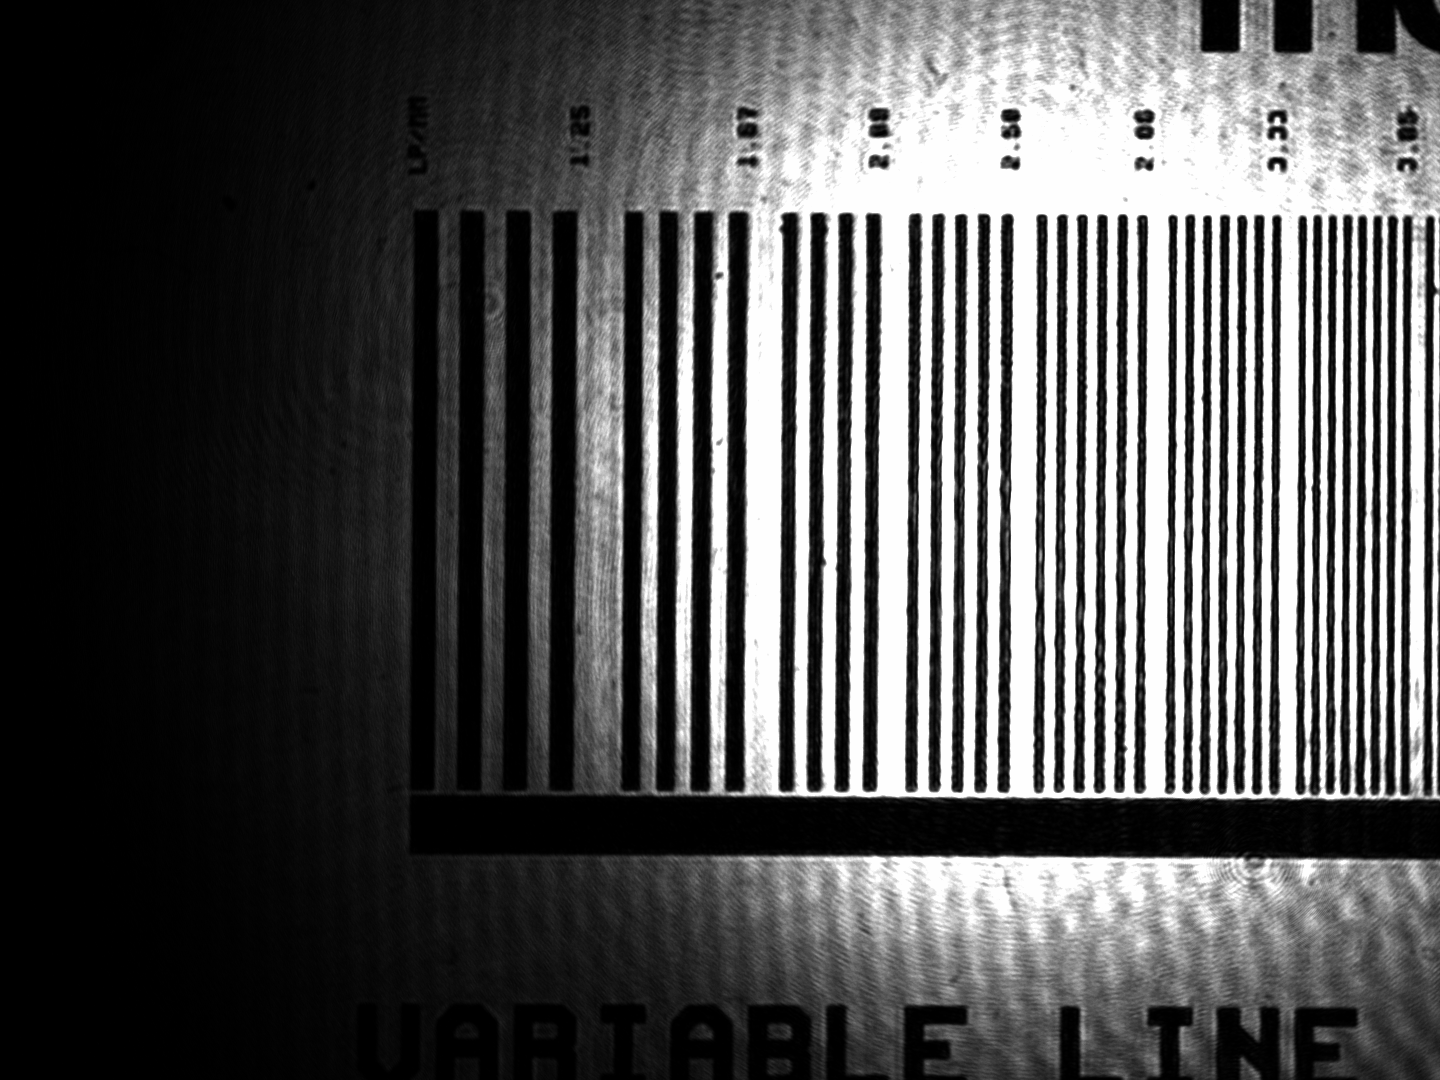
\includegraphics[scale=0.28]{cible_d4_1-7.png}
  \caption{Cible de résolution entre 1.25 et 3.85 mm$^{-1}$ pour un diamètre d'ouverture de l'iris de 2 mm. La fréquence de coupure n'est pas identifiable.}
  \label{cible4-1-7}
\end{figure}

\begin{figure}[H]
  \centering
  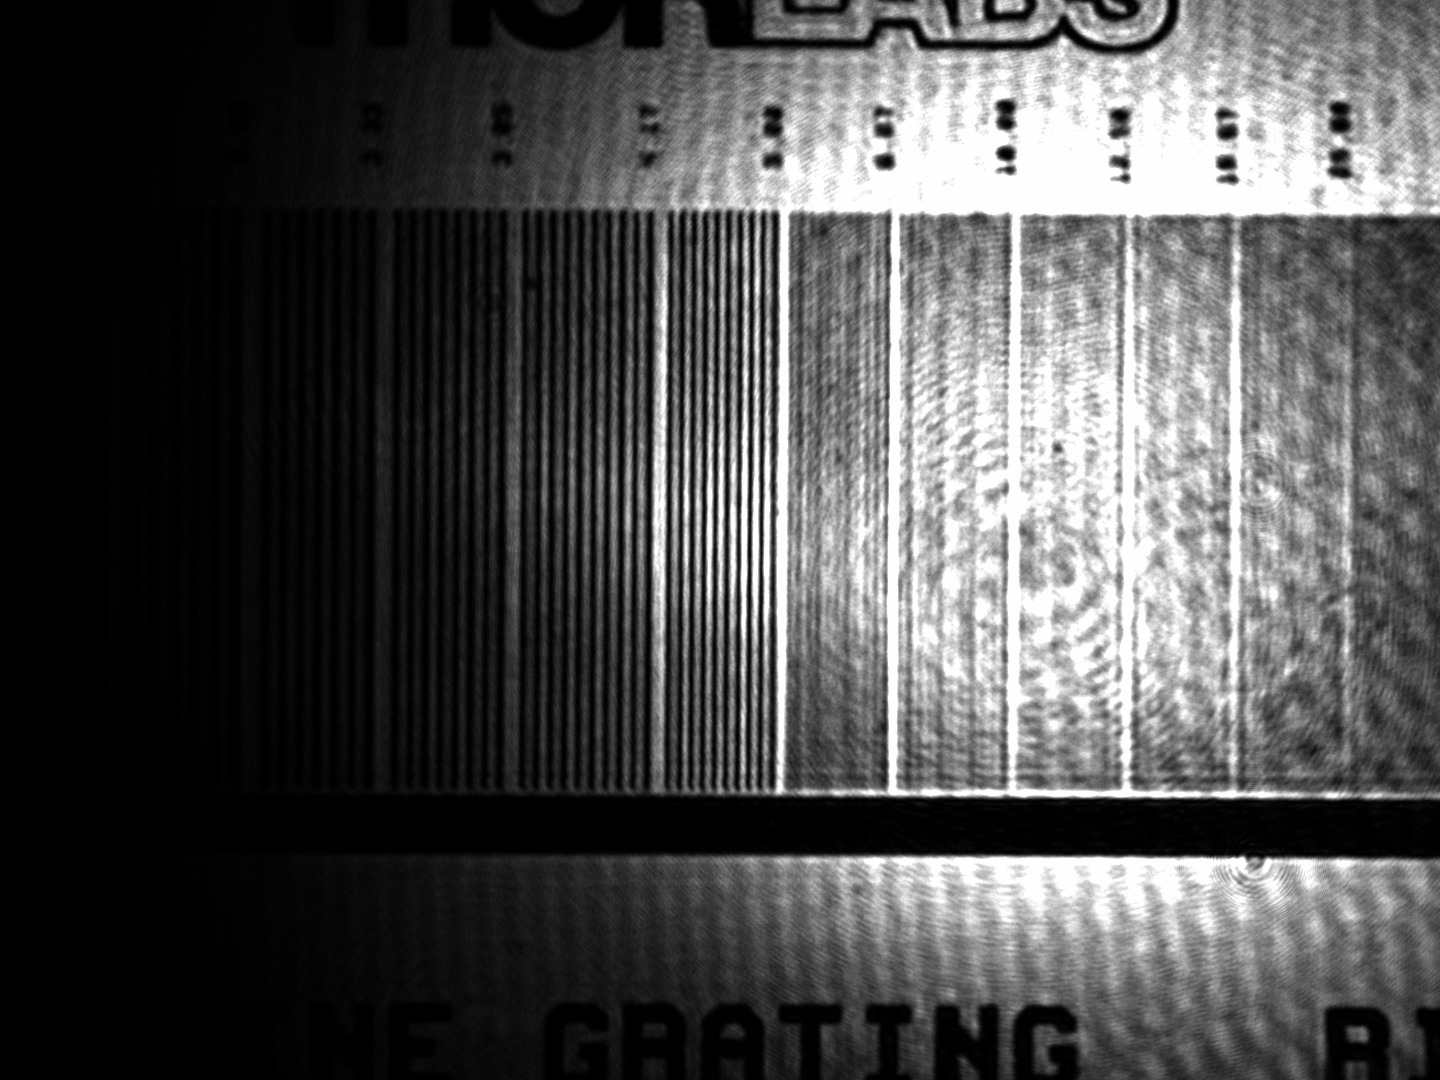
\includegraphics[scale=0.28]{cible_d3_8-14.png}
  \caption{Cible de résolution entre 4.17 et 26 mm$^{-1}$ pour un diamètre d'ouverture de l'iris de 3 mm. La fréquence de coupure est identifiée à 5.88 mm$^{-1}$.}
  \label{cible3}
\end{figure}

\begin{figure}[H]
  \centering
  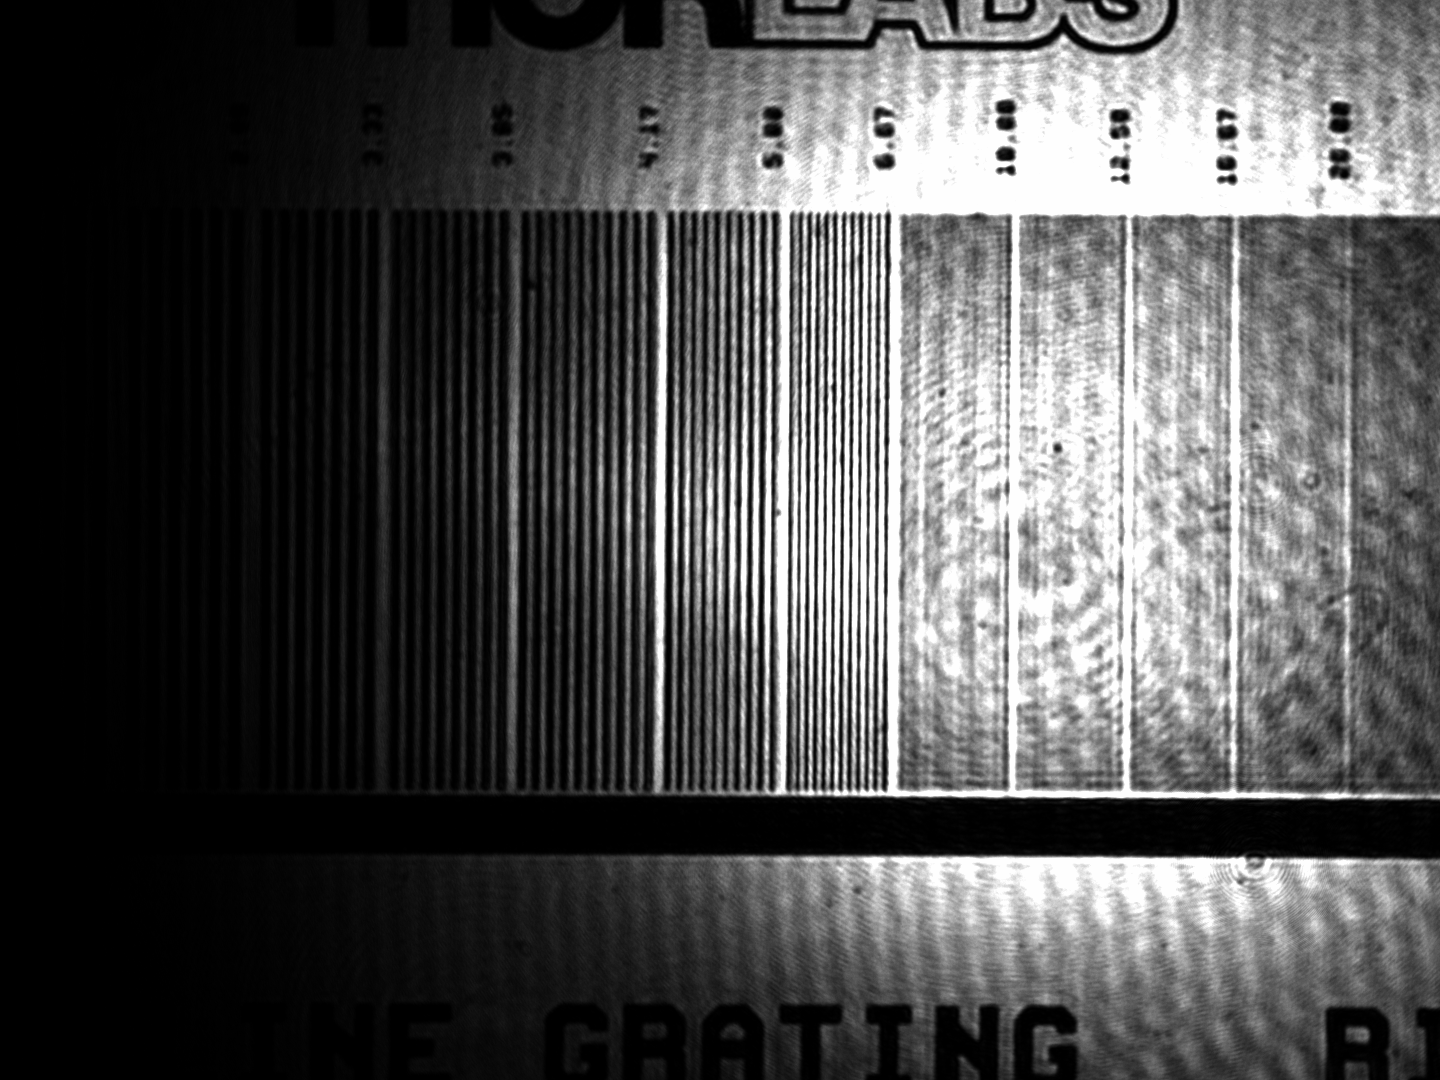
\includegraphics[scale=0.28]{cible_d4_8-14.png}
  \caption{Cible de résolution entre 4.17 et 26 mm$^{-1}$ pour un diamètre d'ouverture de l'iris de 4 mm. La fréquence de coupure est identifiée à 6.67 mm$^{-1}$.}
  \label{cible4-8-14}
\end{figure}

\begin{figure}[H]
  \centering
  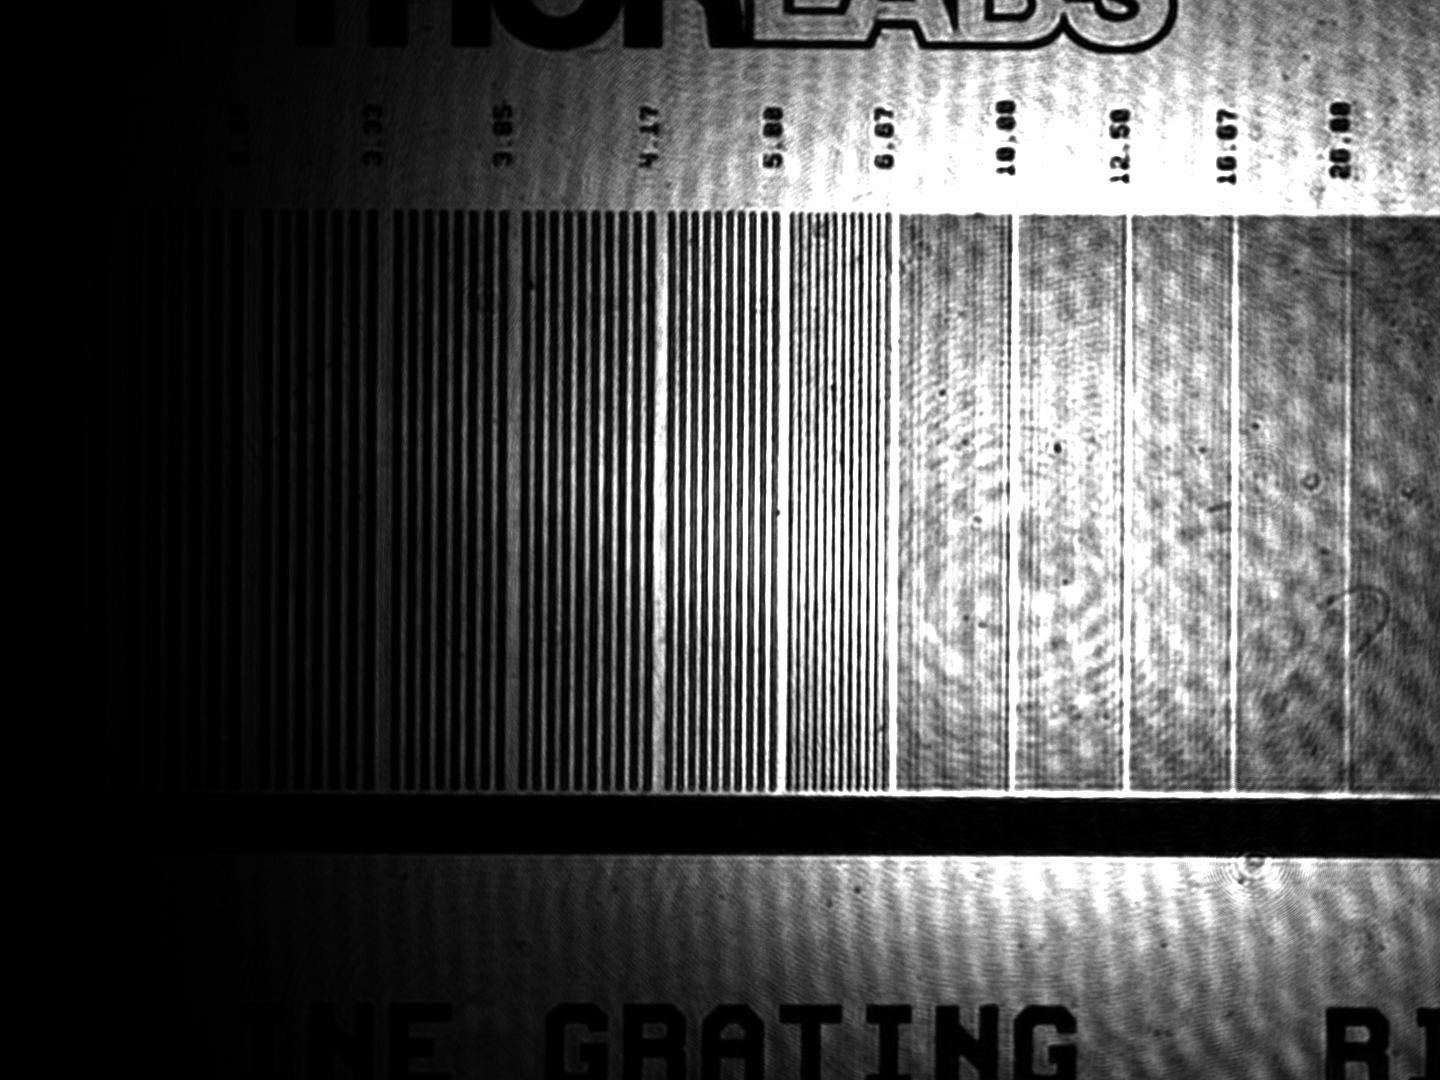
\includegraphics[scale=0.28]{cible_d5_8-14.png}
  \caption{Cible de résolution entre 4.17 et 26 mm$^{-1}$ pour un diamètre d'ouverture de l'iris de 5 mm. La fréquence de coupure est identifiée à 6.67 mm$^{-1}$.}
  \label{cible5}
\end{figure}

\begin{figure}[H]
  \centering
  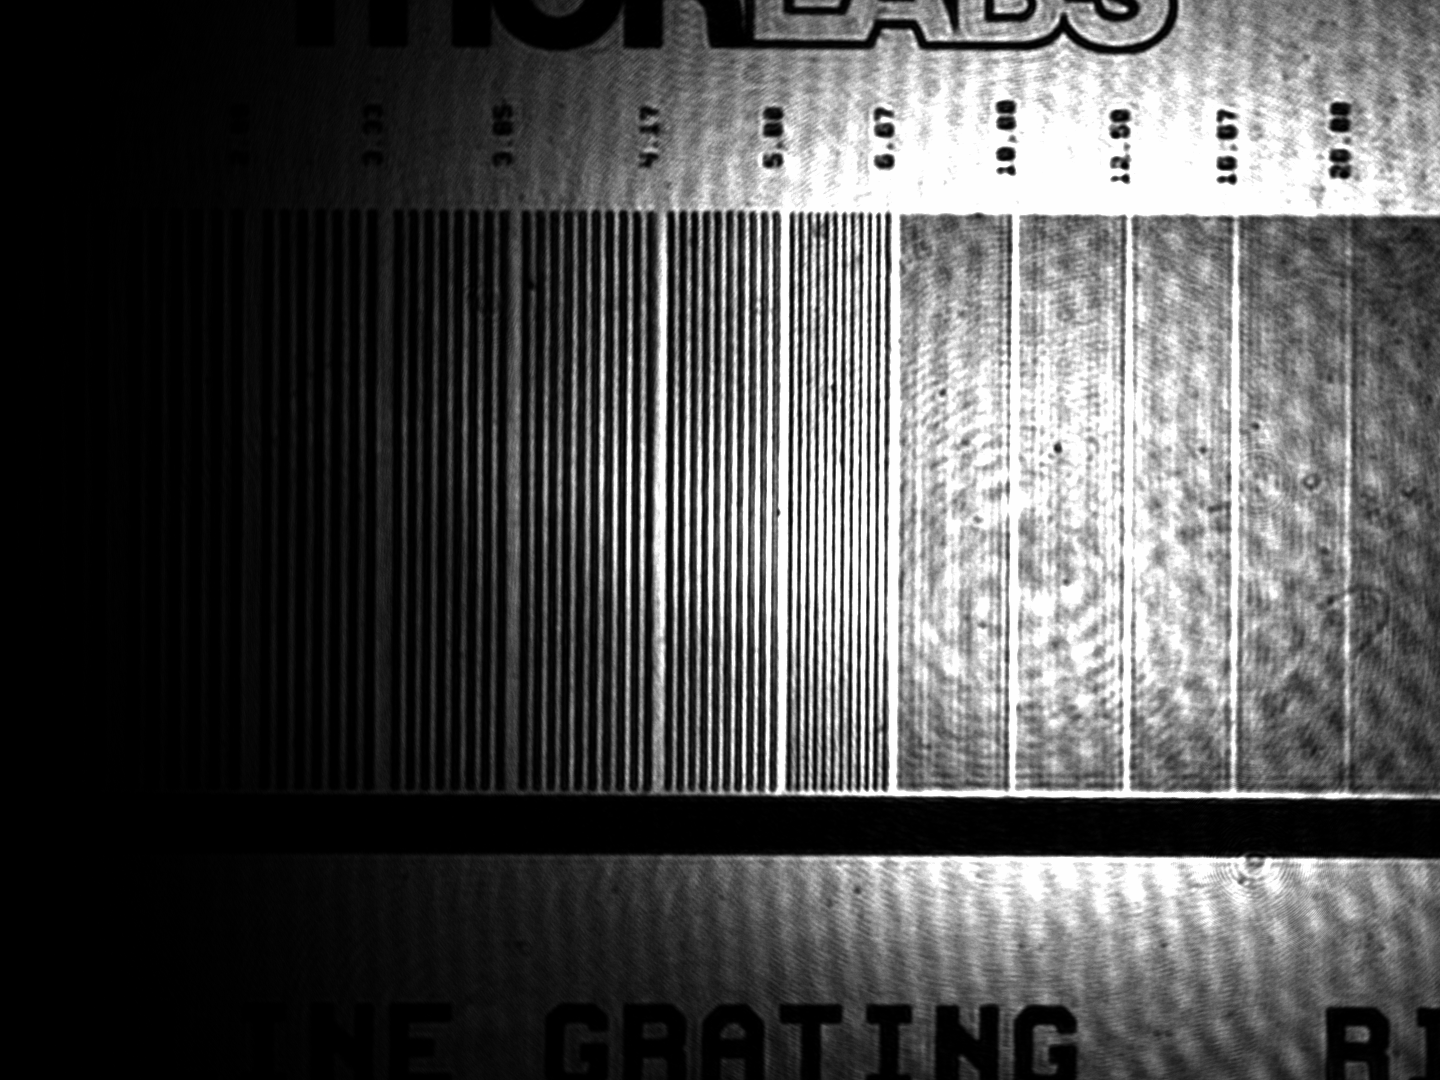
\includegraphics[scale=0.28]{cible_d7_8-14.png}
  \caption{Cible de résolution entre 4.17 et 26 mm$^{-1}$ pour un diamètre d'ouverture de l'iris de 7 mm. La fréquence de coupure est identifiée à 6.67 mm$^{-1}$.}
  \label{cible7}
\end{figure}

\begin{figure}[H]
  \centering
  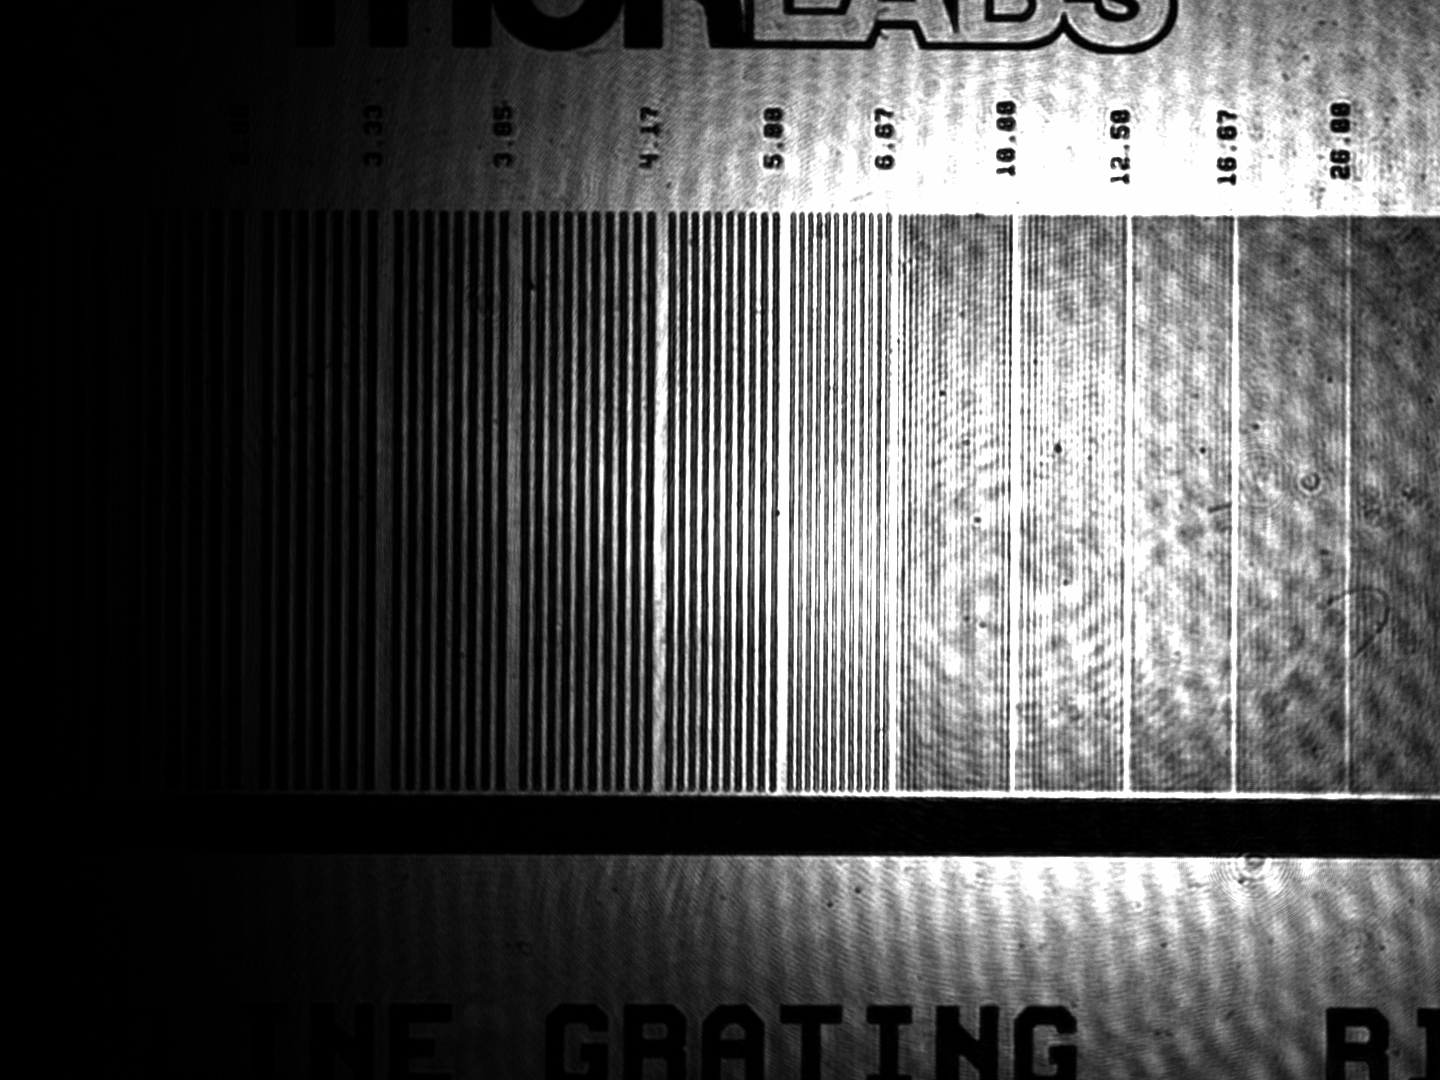
\includegraphics[scale=0.28]{cible_d9_8-14.png}
  \caption{Cible de résolution entre 4.17 et 26 mm$^{-1}$ pour un diamètre d'ouverture de l'iris de 9 mm. La fréquence de coupure est identifiée à 10 mm$^{-1}$.}
  \label{cible9}
\end{figure}

\begin{figure}[H]
  \centering
  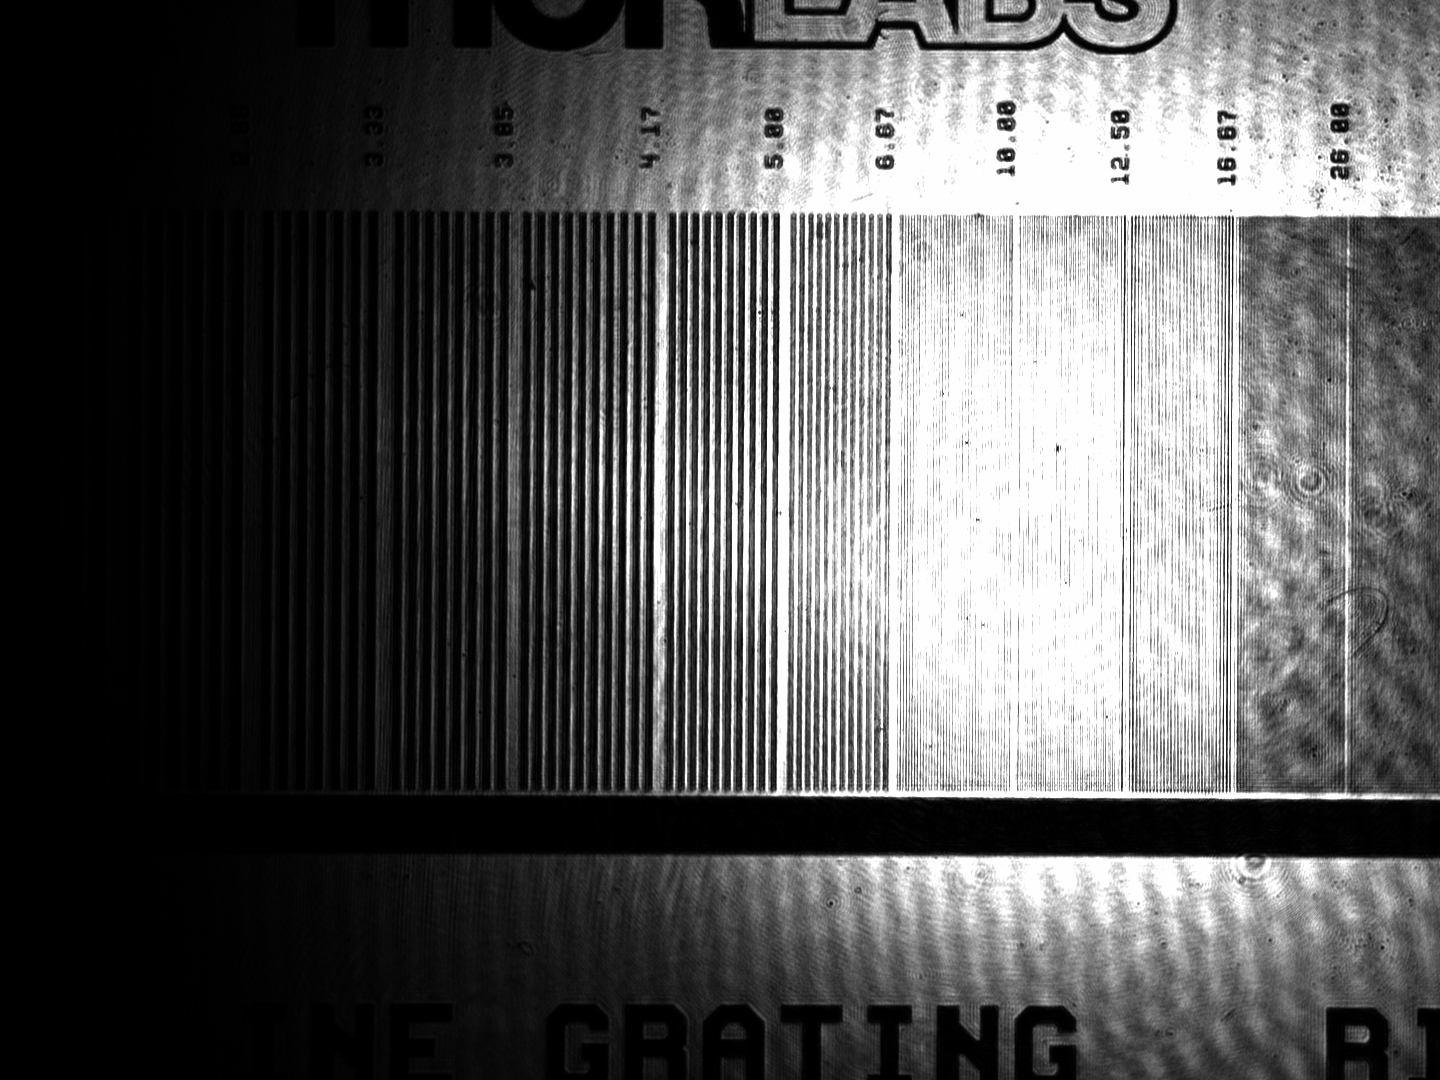
\includegraphics[scale=0.28]{cible_d16_8-14.png}
  \caption{Cible de résolution entre 4.17 et 26 mm$^{-1}$ pour un diamètre d'ouverture de l'iris de 16 mm. La fréquence de coupure est identifiée à 16.67 mm$^{-1}$.}
  \label{cible16}
\end{figure}

\begin{figure}[H]
  \centering
  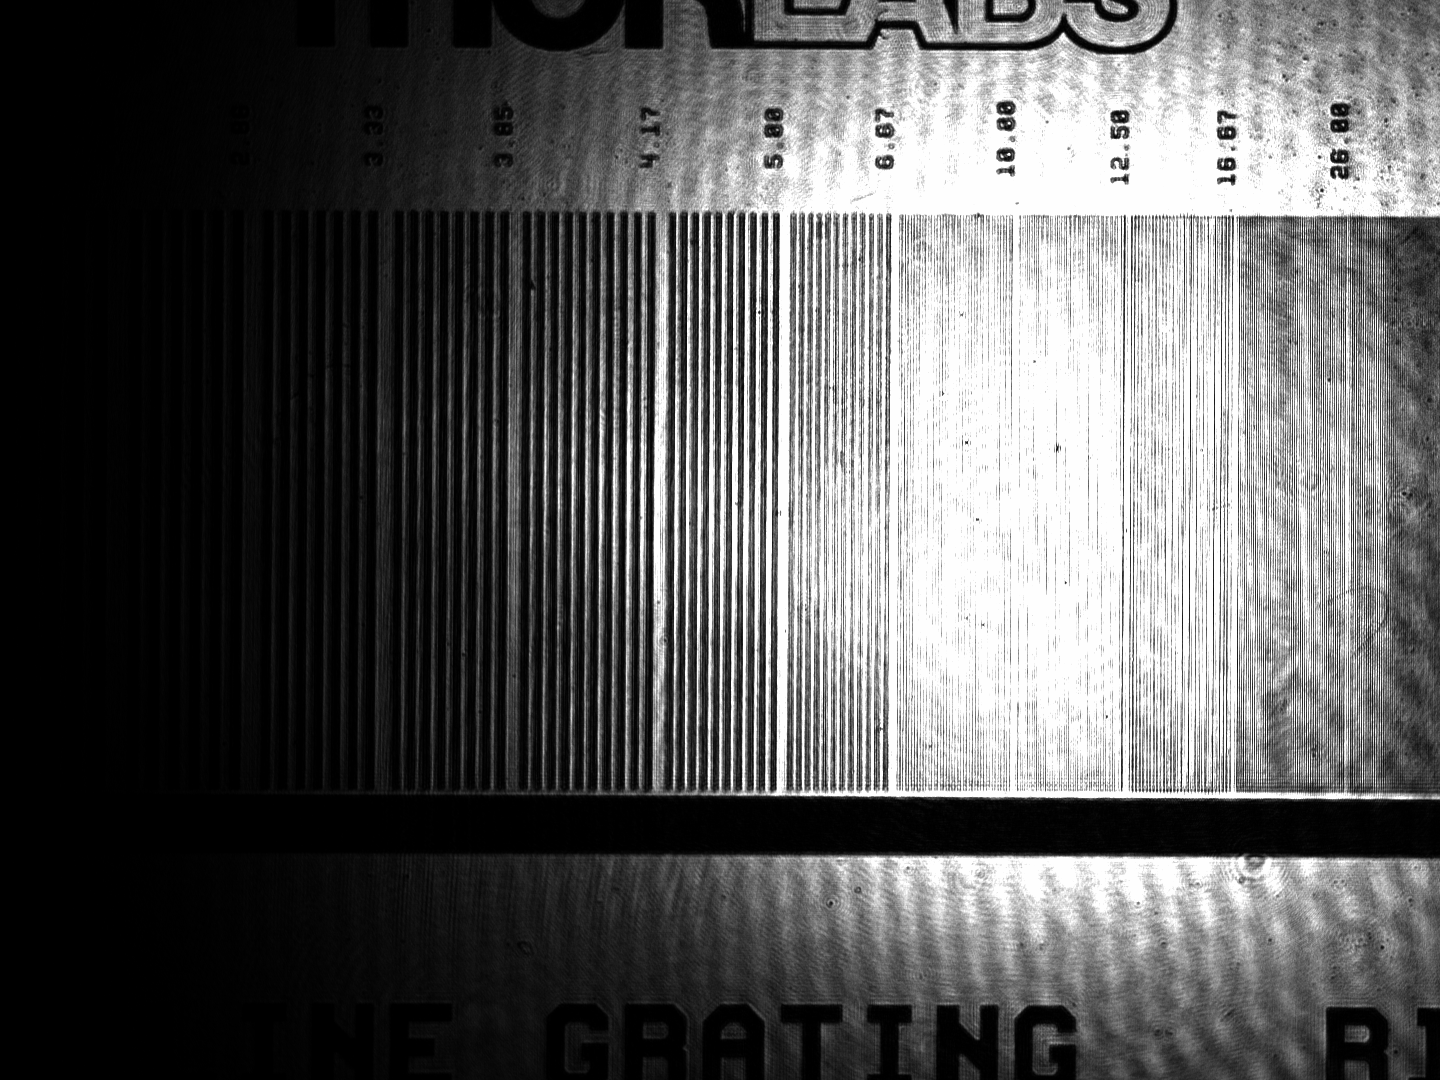
\includegraphics[scale=0.28]{cible_d25_8-14.png}
  \caption{Cible de résolution entre 4.17 et 26 mm$^{-1}$ pour un diamètre d'ouverture de l'iris de 25 mm. La fréquence de coupure est identifiée à 26 mm$^{-1}$.}
  \label{cible25}
\end{figure}

Les fréquences de coupure sont compilées et affichées dans le graphique de la figure \ref{plot}. Les incertitudes sur
le diamètre d'ouverture de l'iris $d$ sont données par la moitié de la plus petite graduation de l'instrument de mesure,
doublée car la mesure se fait à deux points. Cela donne $\Delta d = 1$ mm. Cette incertitude se propage facilement sur
la fréquence de coupure $f_c$  par la méthode des dérivées partielles. Pour cela, il faut la relation théorique entre la
fréquence de coupure et l'ouverture. Cette dernière est dérivée en détail à la section \ref{q1}, elle est :

\begin{equation}
  f_c(d)= \frac{d}{2\lambda f}
\end{equation}

où $\lambda = 632$ nm est la longueur d'onde du laser rouge utilisé et $f = 50$ cm est la focale de la lentille avant le
plan de Fourier, où les filtres sont appliqués. La méthode des dérivées partielles dicte que l'incertitude sur la
fréquence de coupure $\Delta f_c$ est donnée par :

\begin{equation}
  \Delta f_c = \frac{\partial f_c}{\partial d}\Delta d = \frac{\Delta d}{2 \lambda f} \approx 1.58 \text{ mm}^{-1} 
\end{equation}

Ainsi, avec les barres d'erreurs :

\begin{figure}[H]
  \centering
  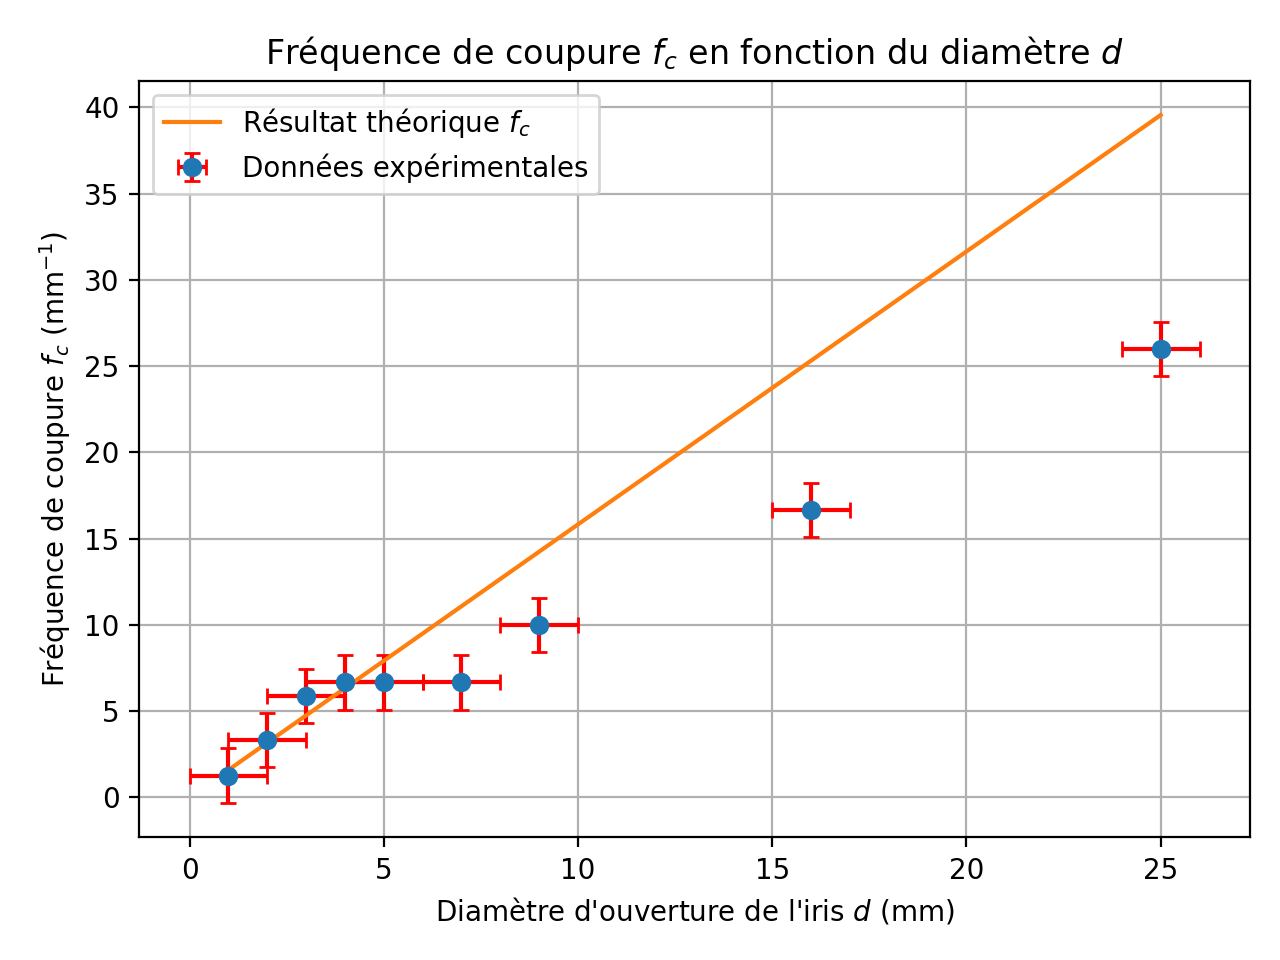
\includegraphics[scale=0.9]{graph_fc.png}
  \caption{Graphique des données expérimentales comparée avec la prédiction théorique. Les incertitudes sur la fréquence
  de coupure sont la propagation des incertitudes du diamètre d'ouverture de l'iris.}
  \label{plot}
\end{figure}



\subsection{Marvin}

Les figures \ref{marvin_min} à \ref{marvin_max} montrent l'application du filtre passe-bas sur la transformée de
Fourier, avec plusieurs diamètres d'iris (donc fréquences de coupure) appliquées.

\begin{figure}[H]
  \centering
  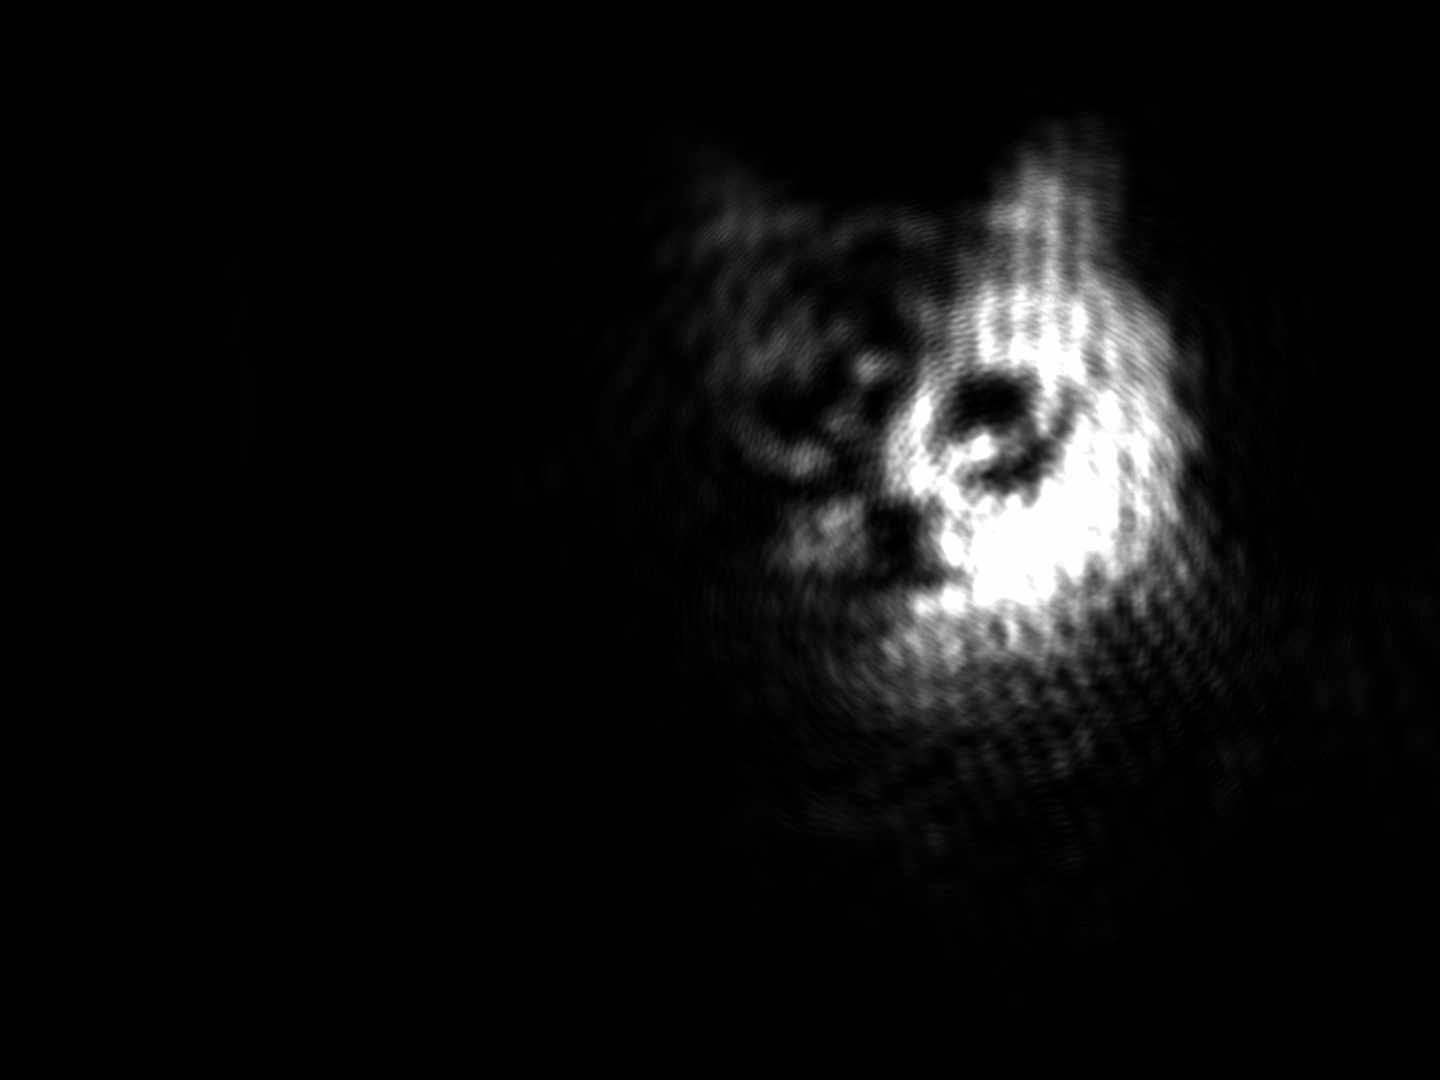
\includegraphics[scale=0.28]{marvin_min.png}
  \caption{Image de l'acétate de Marvin filtrée par l'ouverture minimale de l'iris $d =$ 1.2 mm.}
  \label{marvin_min}
\end{figure}

\begin{figure}[H]
  \centering
  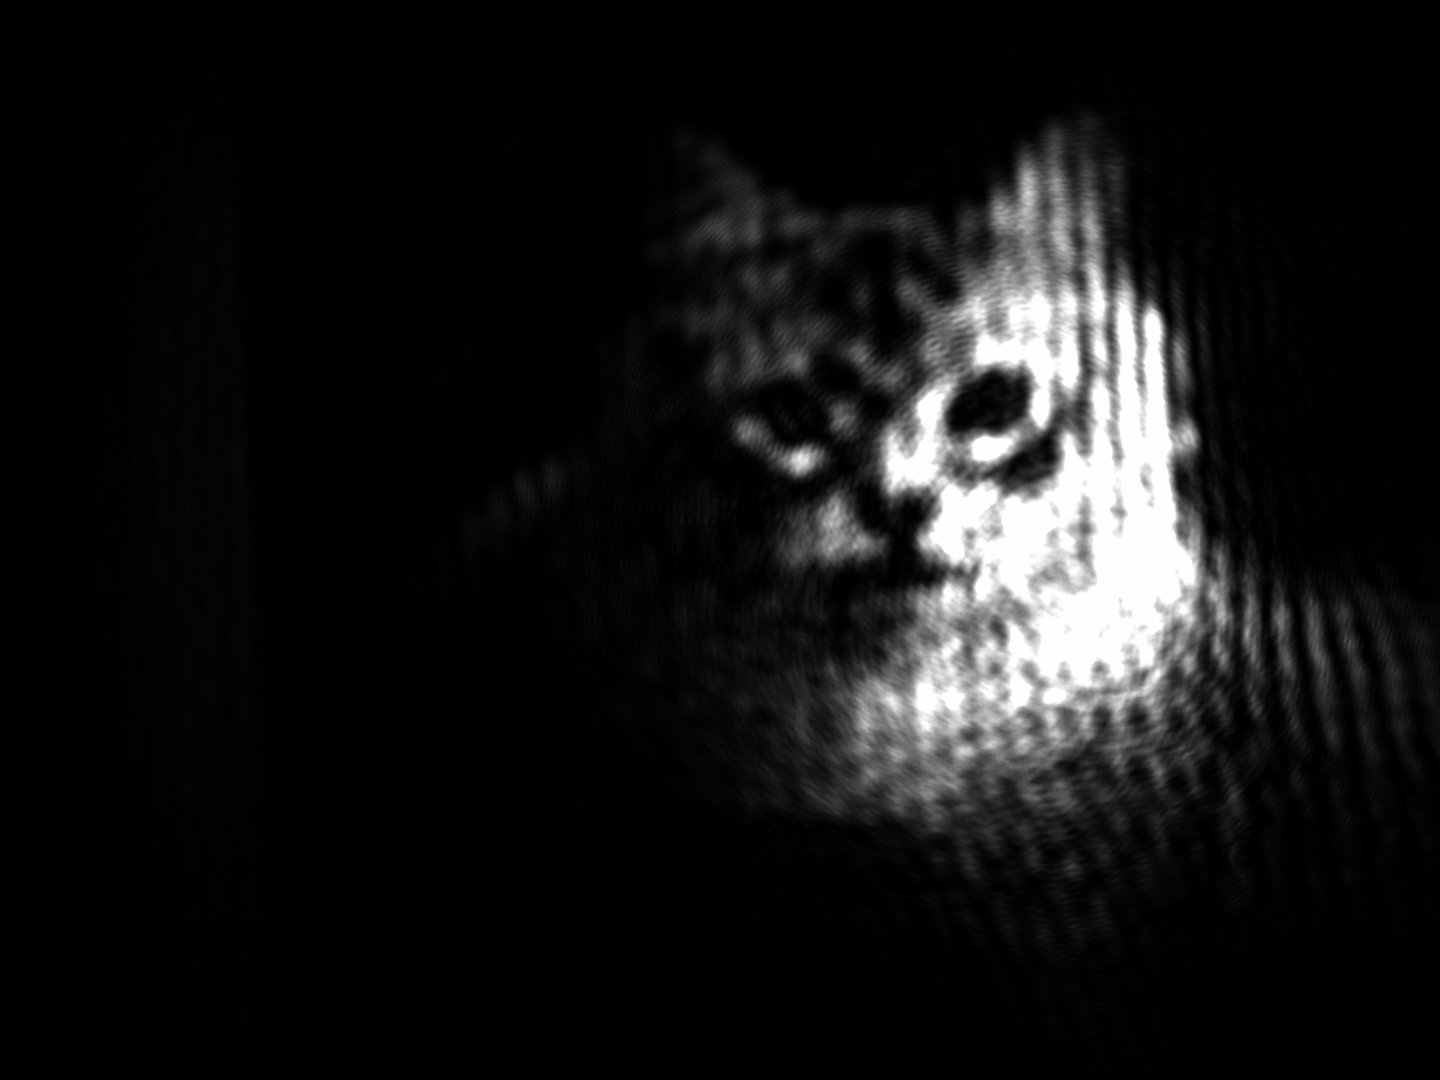
\includegraphics[scale=0.28]{marvin_partiel_d2.png}
  \caption{Image de l'acétate de Marvin filtrée par l'ouverture intermédiaire de l'iris à $d =$ 2 mm.}
  \label{marvin_mid}
\end{figure}

\begin{figure}[H]
  \centering
  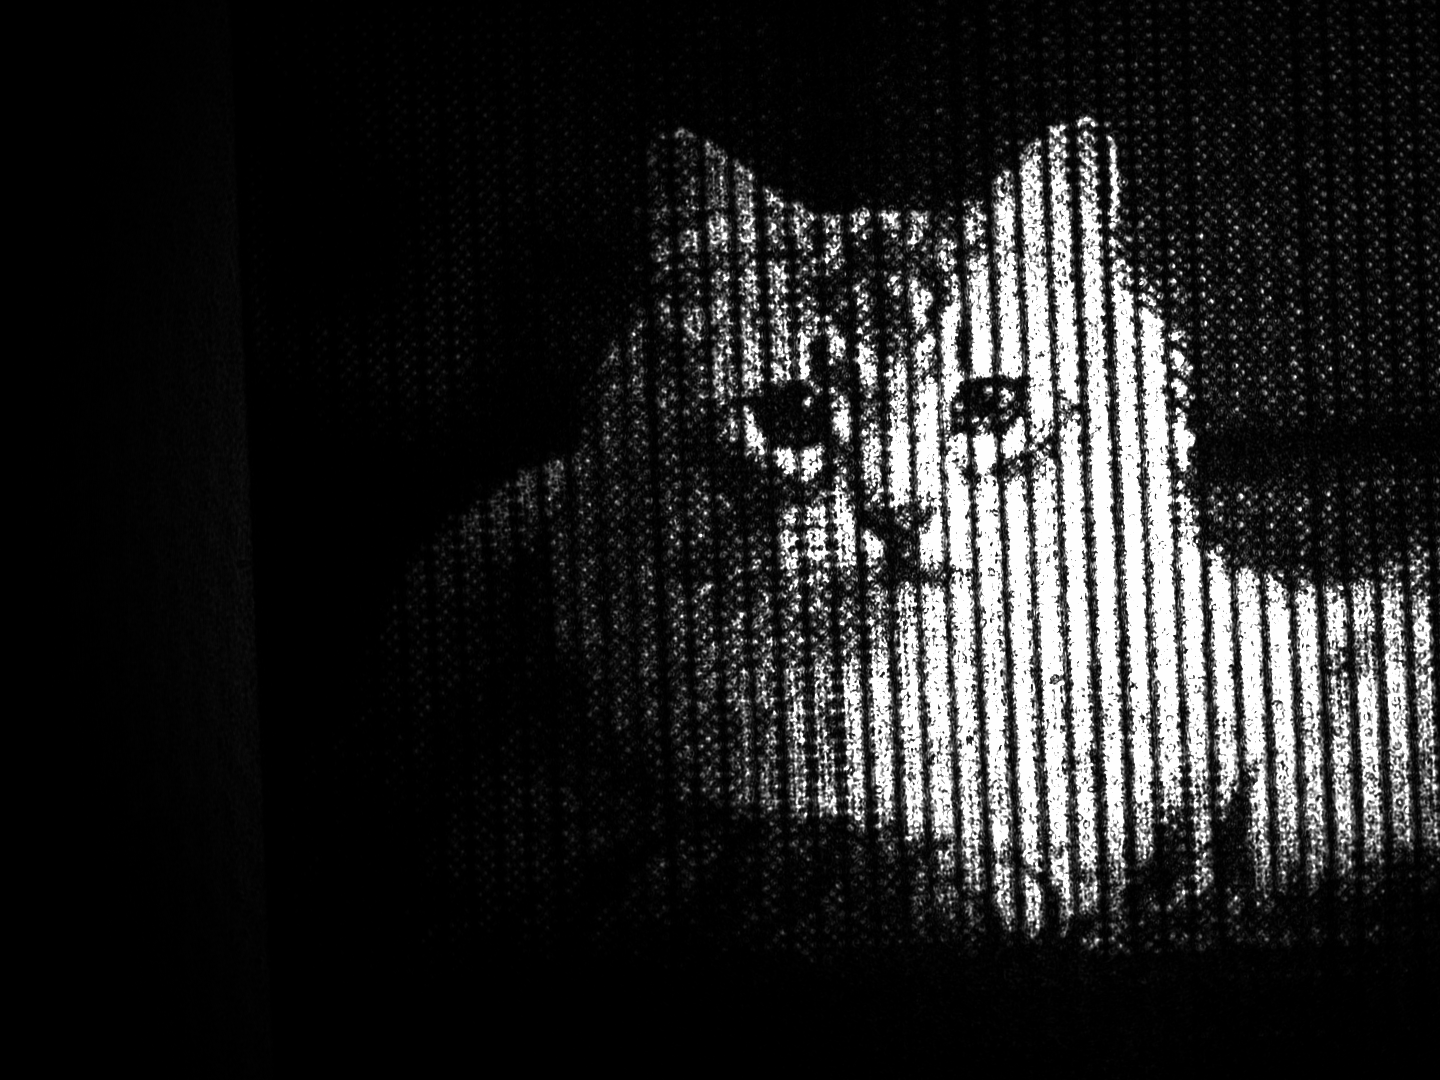
\includegraphics[scale=0.28]{marvin_max_d12-5.png}
  \caption{Image de l'acétate de Marvin filtrée par l'ouverture maximale de l'iris à $d =$ 12.5 mm.}
  \label{marvin_max}
\end{figure}

Il est possible d'observer que le filtre pour enlever les barres verticales fonctionne partiellement pour
une ouverture plus petite, mais a pour conséquece de flouter et d'assombrir grandement l'image. De plus, les 
barres ne sont jamais totalement enlevées.

\section{Discussion}

Afin de comparer les résultats obtenus pour les filtres appliqués sur l'acétate de Marvin avec le modèle théorique,
quelques valeurs de filtres utilisées en laboratoire ont été implémentes sur l'image \texttt{marvin\_striped} avec
un filtre passe-bas top-hat, tel qu'affiché à la figure \ref{cats} :

\begin{figure}[H]
  \centering
  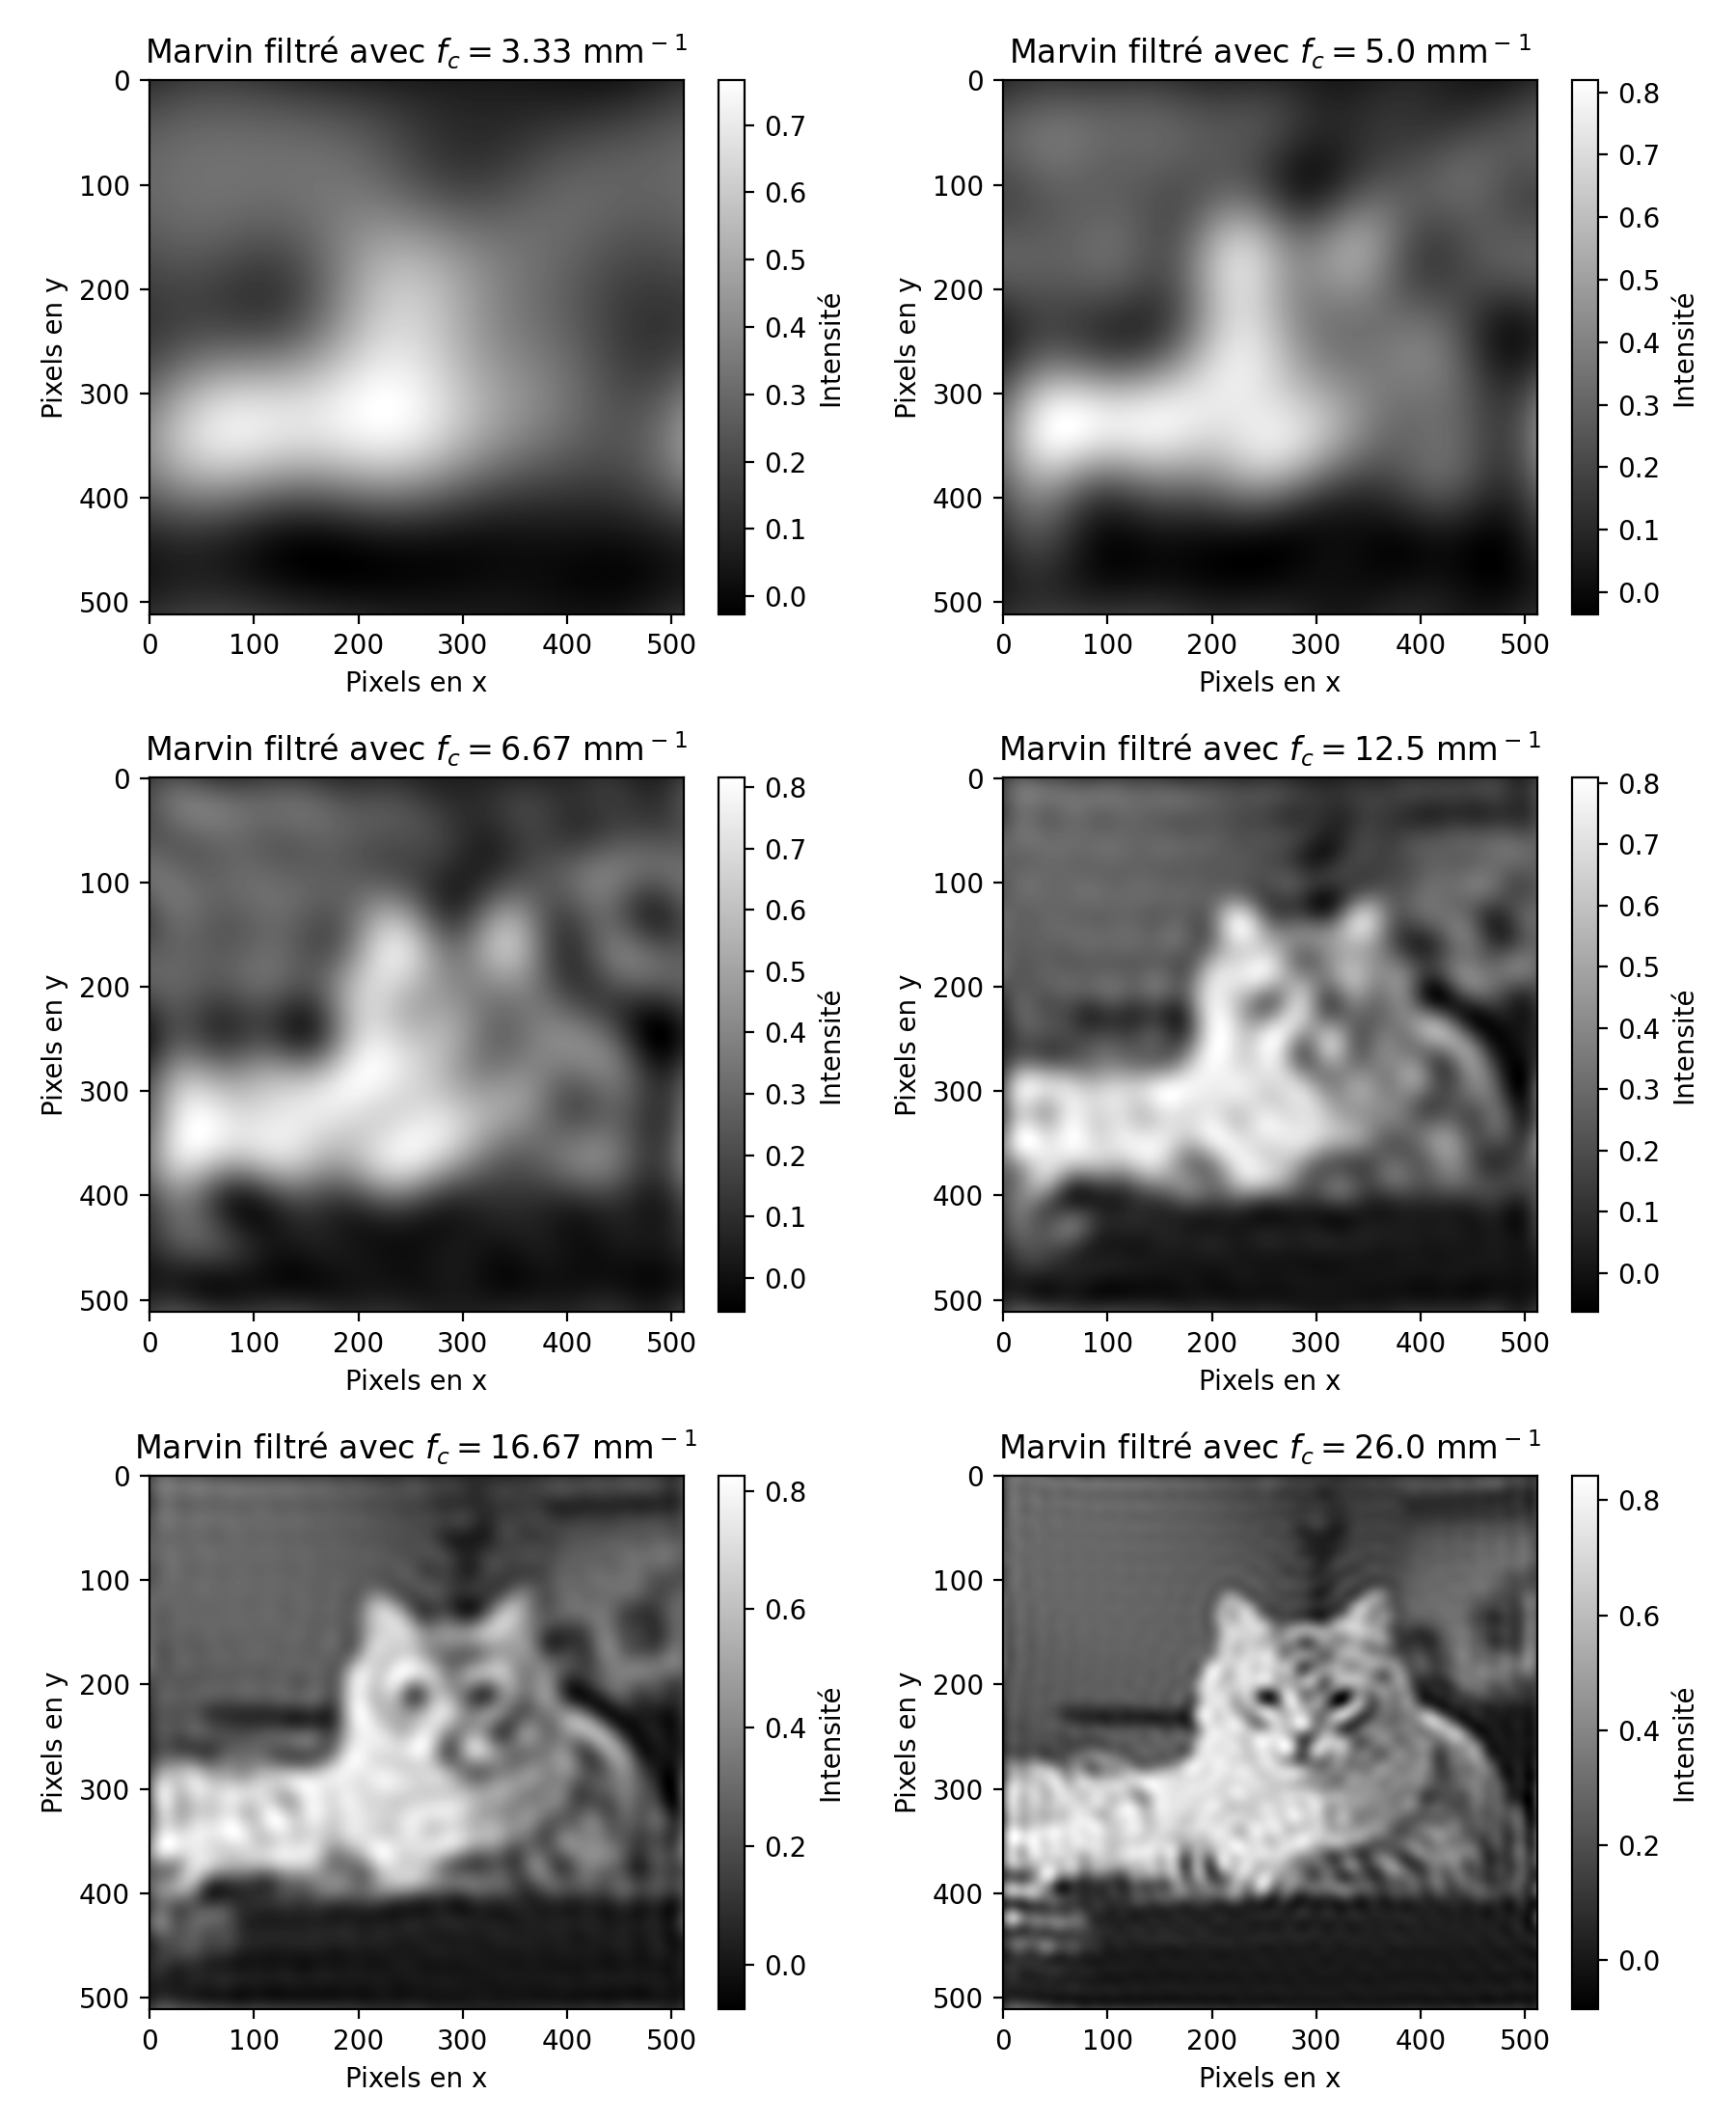
\includegraphics[scale=0.7]{marvin_post_filter_bars.png}
  \caption{Résultat de l'application de filtres top-hat $f_c$ sur l'image de Marvin avec les bandes verticales.}
  \label{cats}
\end{figure}

À titre de référence, l'image originelle de Marvin avec les barres et sa transformée de Fourier sont présentées à la
figure \ref{cat} :

\begin{figure}[H]
  \centering
  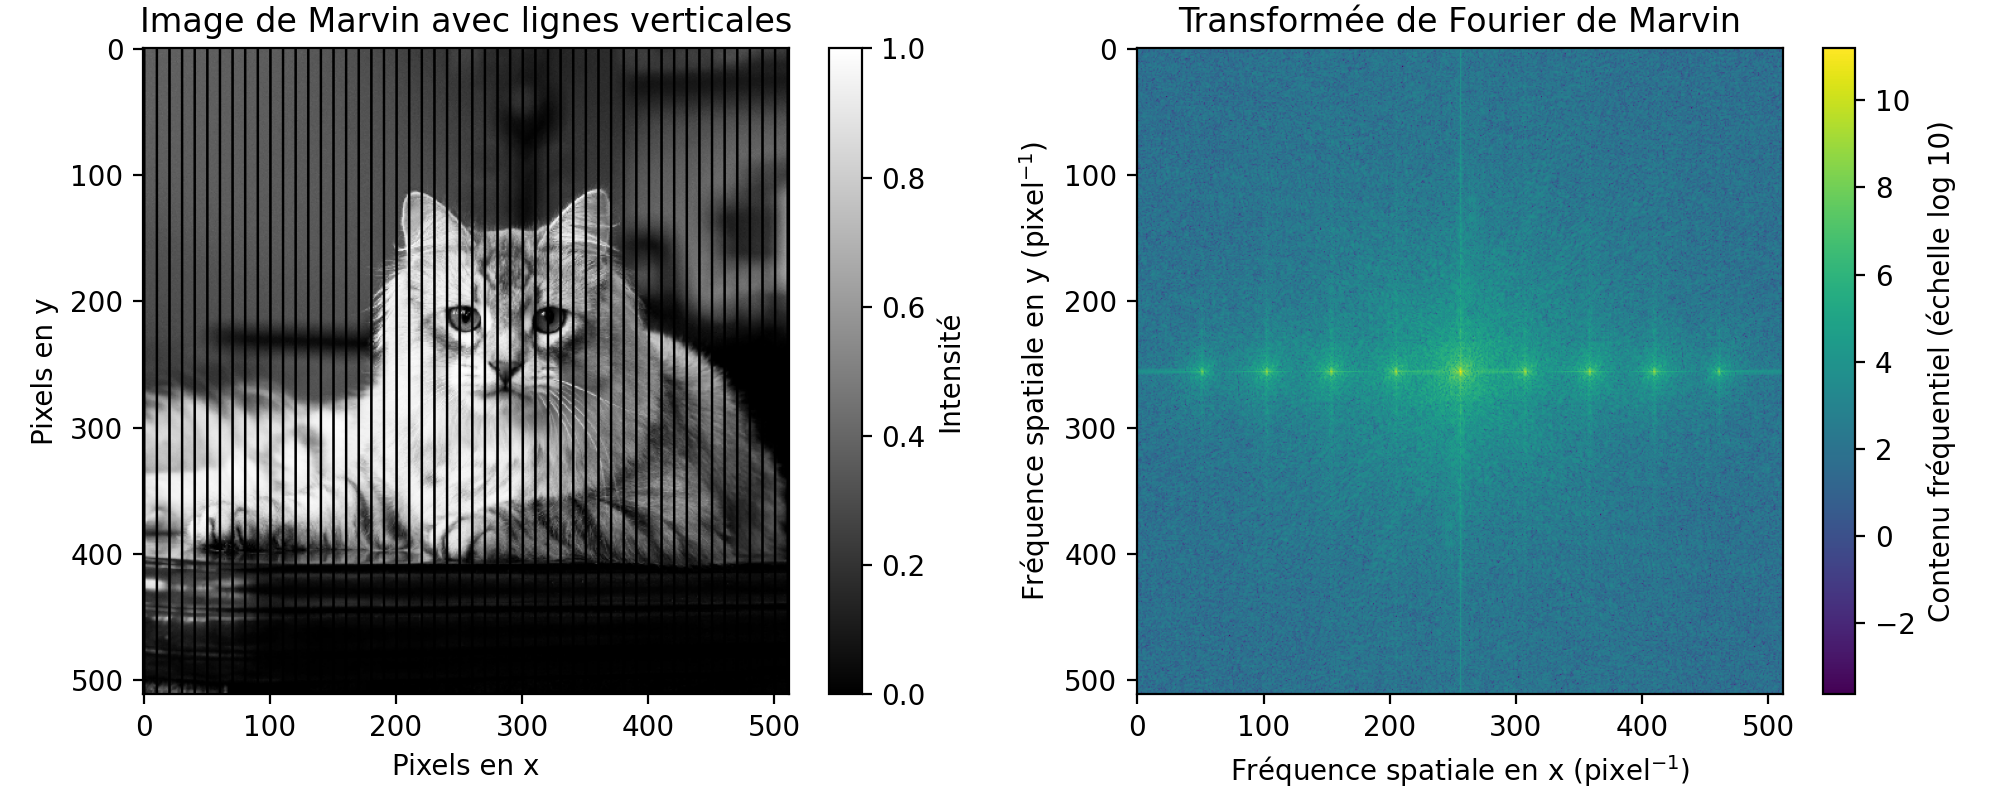
\includegraphics[scale=0.65]{marvin_bars.png}
  \caption{Image originale de Marvin avec les bandes et affichage de sa transformée de Fourier, sur laquelle les filtres
  top-hat sont appliqués}
  \label{cat}
\end{figure}

\subsection{Comparaison entre la théorie et l'expérience}



\subsection{Question 1}\label{q1}

Pour trouver la fréquence de coupure de l'iris selon les paramètres physiques de l'expérience, les deux équations de fréquences spatiales peuvent être utilisées. L'équation pour la fréquence spatiale en $x$ est donnée par :
\begin{equation}
  f_{x}=\frac{x}{\lambda f}
  \label{eqfx}
\end{equation}
Et celle en $y$ est donnée par :
\begin{equation}
  f_{y}=\frac{y}{\lambda f}
  \label{eqfy}
\end{equation}
Où $\lambda$ est la longueur d'onde de la lumière, et $f$ est la longueur focale de la lentille utilisée. Puisque le filtre est de forme circulaire, il est possible de modéliser la fréquence de coupure à l'aide de l'équation d'un cercle, soit la suivante :
\begin{equation}
  x^{2}+y^{2}=r^{2}
  \label{eqcercle}
\end{equation}
Où $r$ correspond au rayon de l'iris. Donc, en isolant les variables $x$ et $y$ dans les équations \ref{eqfx} et \ref{eqfy}, et en remplaçant dans l'équation ci-dessus (Annexe), le résultat suivant est obtenu :
\begin{equation}
  f_{c}=\frac{r}{\lambda f}=\frac{d}{2\lambda f}
  \label{eqfc}
\end{equation}
Ainsi, la fréquence de coupure de l'iris selon les paramètres physiques est donnée par l'équation ci-dessus.

\textcolor{red}{RÉSULTATS COHÉRENTS AVEC THEO?}

\subsection{Question 2}

\section{Conclusion}

\newpage\section*{Annexe}
Avec les équations $f_{x}$ et $f_{y}$, les variables $x$ et $y$ sont isolées, permettant d'obtenir les équations suivantes :
\begin{align*}
  x&=f_{x}\lambda f & y&=f_{y}\lambda f \\
\end{align*}
En remplaçant dans l'équation \ref{eqcercle}, le résultat suivant est obtenu.
\begin{align*}
  (f_{x}\lambda f)^{2}+(f_{y}\lambda f)^{2}&=r^{2} \\
  f_{x}^{2}\lambda^{2}f^{2}+f_{y}^{2}\lambda^{2}f^{2}&=r^{2} \\
  \lambda^{2}f^{2}(f_{x}^{2}+f_{y}^{2})&=r^{2} \\
\end{align*}
En réarrangeant les termes, le résultat suivant est obtenu.
\begin{equation*}
  (f_{x}^{2}+f_{y}^{2})=\frac{r^{2}}{\lambda^{2}f^{2}}
\end{equation*}
Les deux fréquences spatiales $f_{x}$ et $f_{y}$ correspondent à la fréquence recherchée, ainsi l'équation mène à celle \ref{eqfc}, soit :
\begin{equation*}
  f_{c}=\frac{r}{\lambda f}=\frac{d}{2\lambda f}
\end{equation*} 

\clearpage

% \bibliographystyle{unsrtnat}
% \bibliography{My_Library}

\end{document}
